\subsection{Atmospheric Transmission}
\label{introAtmospheric}
For optical signal propagation in the atmosphere, the physical processes dictating the choice of wavelength are summarized in figure\ref{fig:intro_atmosphere} on page\ref{fig:intro_atmosphere}, which illustrate show the effects of the strong absorption by atmospheric gases act to limit transmission to distinct wavelength regions, or spectral bands.With in these bands, the atmosphere is relatively transparent and imaging sensor systems can operate efficiently. For wavelengths longer than about one micro-meter, the dominant absorption is related to excitation of molecular vibrations in water vapor and carbon dioxide. When examined in detail, these processes three distinct transmission windows: the near or shortwave infrared bands(NIR \lambda ~ 0.7 to 1.1 \mu m and SWIR 1.1 to 2.5 \mu m), the midwave IR band(MWIR \lambda ~ 3.3 to 5.0 \mu m), and the long-wave IR band(LWIR \lambda ~ 8 to 14 \mu m).

At the other extreme, for wavelengths much shorter than visible, the same processes responsible for generating airglow limit transmission through the atmosphere. In fact, for wavelengths shorter than ~0.26 \mu m [ultraviolet(UV)], these processes are so strong that no solar radiation reaches the ground and the earth's surface is in perpetual darkness (solar-blind). However, this UV light does propagate for short distances, all owing sensors designed to respond exclusively in this spectral region to detect many man-made emissions. For example, even when pointed directly at the sun, under conditions where a visible or IR system would be completely overwhelmed by the sun's emission, these sensors can detect a UV flash emitted by flames, firearms, or missile plumes. Solar-blind sensors are also of interest because they operate in a region of the spectrum important for detecting certain characteristic florescence associated with biological agents (e.g.,an-thrax) when illuminated by sources operating at even shorter wavelengths. 


\begin{figure}
\centering
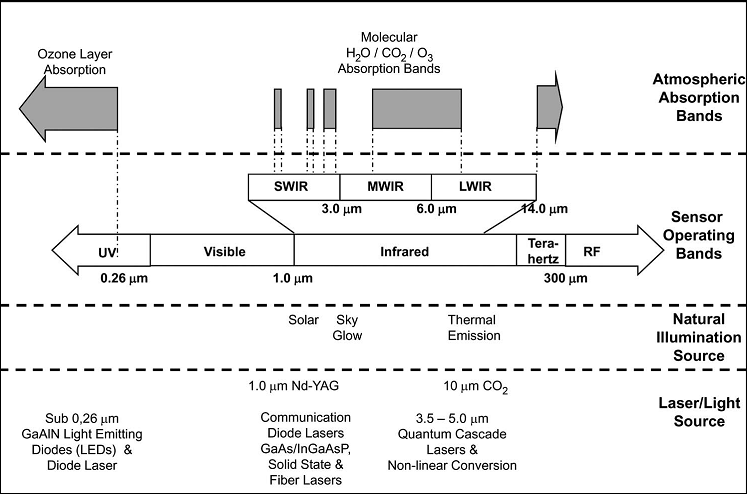
\includegraphics[scale = 1]{chapters/img/intro_atmosphere.jpg}
\caption{A schematic summary illustrating how absorption by various constituents in the atmosphere influences the propagation of light and divides the spectrum into distinct bands.}
\label{fig:intro_atmosphere}
\end{figure}